
\documentclass[conference]{IEEEtran}
\IEEEoverridecommandlockouts
% The preceding line is only needed to identify funding in the first footnote. If that is unneeded, please comment it out.
\usepackage{cite}
\usepackage{float}
\usepackage{placeins}
\usepackage{amsmath,amssymb,amsfonts}
\usepackage{algorithmic}
\usepackage{graphicx}
\usepackage{textcomp}
\usepackage{xcolor}

\def\BibTeX{{\rm B\kern-.05em{\sc i\kern-.025em b}\kern-.08em
    T\kern-.1667em\lower.7ex\hbox{E}\kern-.125emX}}
\begin{document}

\title{Vocal Loudness Estimation and Genre Analysis\\


}

\author{\IEEEauthorblockN{kelian Li}
\IEEEauthorblockA{\textit{Center for Music Technology} \\
\textit{Georgia Institute of Technology}\\
Atlanta, USA \\
kli421@gatech.edu}
\and
\IEEEauthorblockN{Alexander Lerch}
\IEEEauthorblockA{\textit{Center for Music Technology} \\
\textit{Georgia Institute of Technology}\\
Atlanta, USA \\
alexander.lerch@gatech.edu}
}

\maketitle

\begin{abstract}
This paper proposes a method to estimate the isolated vocal loudness from the mixture signal. This data-driven machine learning approach is based on the Support Vector Regression (SVR) model. Trained on the pre-measured vocal loudness and the audio features of the mixture signal, the model is able to estimate the vocal loudness in any songs. An analysis of vocal loudness by genres are later performed on the estimated output of the model.
\end{abstract}

\begin{IEEEkeywords}
audio information retrieval, automatic mixing, intelligent music production 
\end{IEEEkeywords}

\section{Introduction}

Loudness, manipulated by gain knobs and  faders, is the most important factor that influences the listeners' perception of one instruments in the mix. The vocal is commonly the most present sound source in popular music, as it is sometimes referred as "the money track". Thus, understand the vocal loudness is the vital part of understand the mixing process as we work towards automatic mixing.

Automatic mixing is a relative new research field \cite{de2017ten} \cite{de2019intelligentmusic} \cite{moffat2019approaches}. The development of automatic mixing requires understanding the mixes created by professional human engineers. In \cite{wilson2016variation}, Wilson and Fazenda present an analysis of 1501 mixes, over 10 songs, created by amateur mixing engineers. Man et al. in \cite{man2014analysis} conduct a mixing experiment and audio analysis on eight songs are each mixed by eight professional engineers. However neither of the two studies can be scaled up to truly understand the professional mixing procedure. In order to approach automatic mixing statistically on large professional mixes, the analysis needs to be conducted on mixture signals because the digital audio workstation sessions and multi-tracks are not publicly unavailable.


\section{Related Works}

Research on automatic audio feature and mixing parameter extraction of individual tracks from the mixture signal is largely unexplored. In \cite{barchiesi2010reverse}, Barchiesi and Reiss proposed a method to retrieve the mixing parameters by least-squares optimization. However, this method requires the multi-tracks available. 

The recent preceding by Uhle et al. \cite{uhle2021clean} uses Deep Neural Networks (DNN) to measure the clean dialogue momentary loudness with the presence of background sounds. They report a mean absolute error (MAE) of  0.5 dB for short-term loudness estimation computed from the momentary loudness. However, this model cannot be directly applied to singing vocal loudness estimation in music for two reasons. Firstly, the training and validation data are random uncorrelated pairs of speech and background signals. But in music, singing vocals and the accompaniment tracks are usually correlated. Secondly, the validation signal are created by mixing speech and background signals at signal-to-noise ratios (SNRs) of \{0, 6, 12, 18\} dB. The SNRs in music are usually lower than these 4 fixed ratios.
\section{Method}

With the isolated vocal tracks and accompaniment tracks available, the target vocal loudness values can be obtained before mixing the two. A set of audio features are then extracted from the mixture signal. Using the audio features as the input, the supervised learning model is able to learn the relation of the features and the target vocal loudness. And finally, after the training process, the model can predict the vocal loudness given the audio of any songs without the isolated vocal track.

Support vector regression (SVR) model \cite{drucker1997support} is a commonly used machine learning model for regression problems. SVR is chosen because of several advantages: (1) The prediction error of SVR is low; (2) The SVR model has good generalization capability; (3) The computational complexity of SVR increases linearly with the number of features \cite{awad2015support}.


\subsection{Model Input}

The audio signals are sliced into overlapped segments of 3 seconds length with the hop size of 100 ms following the EBU recommendation of short-term LUFS \cite{ebu2011loudness}. Prior study suggests that more sophisticated psychoacoustic loudness models do not lead to better results in automatic level adjusting \cite{wichern2015comparison}. The loudness values for the training data are computed using Essentia library's implementation of short-term LUFS \cite{bogdanov2013essentia}. 

The input features to the SVR model are the first 20 Mel-Frequency Cepstrum Coefficients (MFCC), 128 VGGish \cite{hershey2017cnn} embeddings, and the short-term loudness of the mixture signal. The total 149 features for each 3-second audio segment are normalized by Z score transformation.

MFCCs are considered the standard audio features for classification tasks. The 20 MFCCs are computed by the Librosa library \cite{mcfee2015librosa} with the window size of 1024 samples and the hop size of 512 samples and averaged over the 3-second length. 

The publicly-released VGGish model \cite{hershey2017cnn} has been trained on 8M-YouTube dataset for audio classification, and is used to generate high-level abstract feature embeddings from audio for other downstream tasks. The input signals are down-sampled to 16kHz as required by the VGGish model. 128 VGGish embeddings of in the window of 1 second with a hop size of 100 ms are computed from this pre-trained Deep Neural Network. The embeddings are averaged over the 3-second length. 

Because the mixture loudness can be measured directly from the audio signal, estimating the relative vocal loudness (vocal-to-mixture ratio) is equivalent to estimating the absolute vocal loudness. The target vocal loudness values are transformed from the absolute short-term loudness to the loudness difference compared with the mixture loudness, 
\begin{equation} \label{eq1}
STL_{\Delta vox}  =  STL_{vox} - STL_{mixture}
\end{equation}
where $STL_{\Delta vox}$ is the relative vocal loudness, $STL_{vox}$ is the short-term loudness of the vocal signal, and $STL_{mixture}$ is the short-term loudness of the mixture signal. 

The next step is to truncate the relative vocal loudness values below -15 dB to be -15 dB. The main vocal is merely mixed in this level which is nearly inaudible in common listening level.
\begin{equation}
  STL_{\Delta vox} = \left \{
  \begin{aligned}
    &STL_{\Delta vox}, && \text{if}\ STL_{\Delta vox} > -15dB \\
    &-15 dB, && \text{otherwise}
  \end{aligned} \right.
\end{equation} To reduce the range of the target values, the relative vocal loudness in the range of $(-\infty, 0]$ dB is converted to relative amplitude in the range of $[0, 1]$,
\begin{equation} \label{eq2}
A_{\Delta vox} = 10^{\frac{STL_{\Delta vox}}{20}}
\end{equation}
where $A_{\Delta vox}$is relative vocal loudness in amplitude, and $STL_{\Delta vox}$ are as defined in (1). This method yields better results than min-max normalization.

\subsection{Model Output}
The estimated relative vocal loudness in amplitude is transformed back to dB  scale,
\begin{equation} \label{eq3}
\hat{STL_{\Delta vox}} = 20  \; log_{10}(\hat{A_{\Delta vox}})
\end{equation}
where $\hat{STL_{\Delta vox}}$ is the estimated relative vocal loudness, and $\hat{A_{\Delta vox}}$ is the estimated relative vocal loudness in amplitude.

The relative accompaniment loudness (acc) as a side task is estimated using the same method.

\subsection{Model Training}

The accompaniment loudness is estimated first, then the estimated values are fed into the model as a feature for vocal loudness estimation. Using the implementation from scikit-learn library \cite{scikit-learn}, the SVR model is trained with C=1, epsilon=0.1, gamma = 0.001, and Radial Basis Function (RBF) Kernel.

\subsection{Frequency Band Energy Estimation}
Using the same method and hyper-parameters, the model is trained for the task of vocal frequency band estimation. Following the method proposed in \cite{hafezi2015autonomous}, the filter bank consists of 10 second order Butterworth bandpass filters. The center frequencies are [31.5, 63, 125, 250, 500, 1K, 2K, 4K, 8K, 16K] Hz. The RMS of the filtered signal is calculated for each 3-second segment as the  target values.

\section{Evaluation}
\subsection{Data}
Audio signals for training and testing were generated by mixing recordings of the singing vocal tracks and the accompaniment tracks. The vocal tracks are scaled down by random gains in the range of uniformly distributed [0, -6] dB from the original signal. Stereo signals are down-mixed to mono signals. The references for target loudness values are computed on the original clean signal. 

The training data is collected from the MUSDB18HQ dataset\cite{MUSDB18HQ}. The MUSDB18HQ dataset contains 150 full lengths high-quality music tracks (about 10h duration) in 44.1 kHz of different genres in Western popular music along with their original clean vocals, drums, bass, others stems, and the accompaniment tracks. The actual training data is a subset of the MUSDB18HQ dataset which includes 3492 non-overlapped 3-second audio segments and approximately 3h total duration, 30\% of the full dataset. Increasing the training data size does not lead to better results.

The testing and validation data is collected from MIR-1K dataset\cite{hsu2009improvement}. The MIR-1K dataset consists of 110 karaoke Chinese pop songs (133 min duration, about 1 min in average for each song) in 16 kHz which contain the clean vocal tracks and the accompaniment tracks. There are 19 amateur singers in total, and the audio is not professionally recorded or mixed.


\subsection{Baseline System}
The baseline system outputs the mean values of vocal loudness in the training data as the estimation,

\begin{equation} \label{eq4}
 \hat{STL_{\Delta mean}}  = \frac{1}{n}\sum_{n=1}^{\infty} {STL_{\Delta vox}}_{[n]} \
\end{equation}where $\hat{STL_{\Delta mean}}$ is the output of the baseline system, and ${STL_{\Delta vox}}_{[n]}$ is the relative vocal loudness of each audio segment in the training data.

\subsection{metrics}
The metric of the evaluation is Mean Absolute Errors (MAEs) and Maximum Errors (MEs). The evaluation performs on each file of the validation set at first, and the average MAE and ME of all files are calculated afterwards.



\section{Results}

\subsection{Loudness Estimation}



\FloatBarrier
\begin{figure}[h]
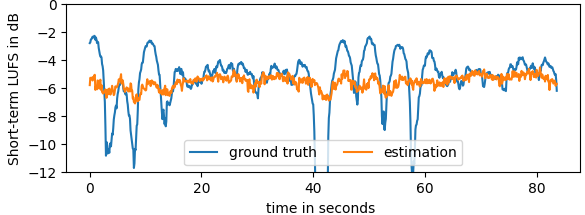
\includegraphics[width=8cm]{02 vox.png}
\centering
\caption{SVR relative vocal loudness estimation (epslion = 0.3)}
\end{figure}
\FloatBarrier

\FloatBarrier
\begin{figure}[h]
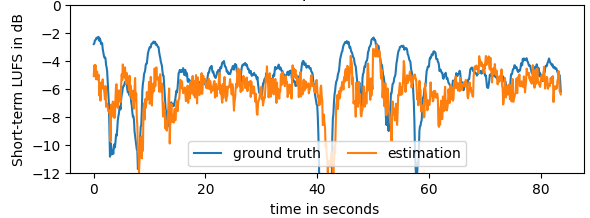
\includegraphics[width=8cm]{01 vox.png}
\centering
\caption{SVR relative vocal loudness estimation (epslion = 0.1)}
\end{figure}
 \multicolumn{4}{l}{$^{\mathrm{*}}$The baseline system.}
\FloatBarrier
Figure 1 and figure 2 (the proposed model) show the SVR vocal loudness estimation of one track with different epsilon parameters. The epsilon parameter determines the epsilon-tube width. The data points inside of the tube are considered as correct predictions which which no penalty is associated. When epslion = 0.3, the estimation MAE is 1.36 dB, 0.19 dB lower than the MAE of 1.55 dB in the case of epslion = 0.1. However, figure 1 and figure 2 indicate that the model with higher epslion value may only make good predictions within a very small loudness range. 


\FloatBarrier
\begin{figure}[h]
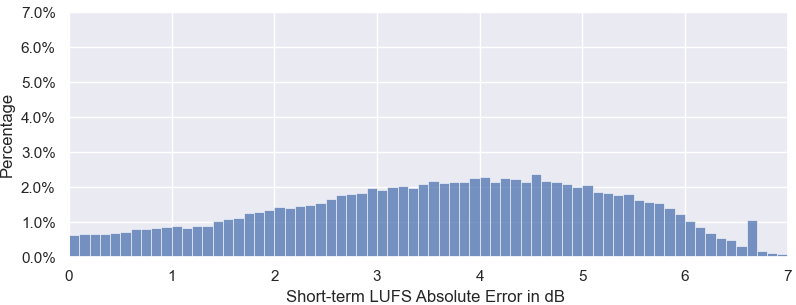
\includegraphics[width=8cm]{Mean_histogram vox.png}
\centering
\caption{Mean Value vocal loudness estimation error histogram}
\end{figure}
\FloatBarrier

\FloatBarrier
\begin{figure}[h]
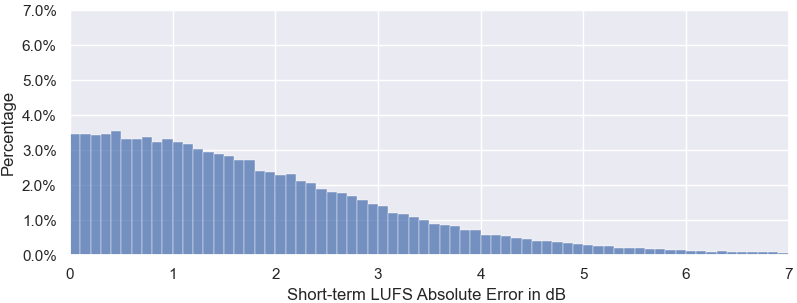
\includegraphics[width=8cm]{SVR_histogram vox.png}
\centering
\caption{SVR vocal loudness estimation error histogram}
\end{figure}
\FloatBarrier

\FloatBarrier
\bgroup
\def\arraystretch{1.3}% 
\begin{table}[h]
\centering
 \caption{Results of the vocal and accompaniment loudness estimation}
 \begin{center}
\begin{tabular}{l*{6}{c}r}
\hline
\hline
              & \textbf{VOX MAE(dB)} & VOX ME & ACC MAE & ACC ME \\
\hline
Mean Value$^{\mathrm{*}}$  & 3.65 & \textbf{6.35} & 1.17 & 3.65  \\
 SVR & \textbf{1.86} & 7.12 & \textbf{1.00} & \textbf{3.12}  \\
 \hline
\multicolumn{4}{l}{$^{\mathrm{*}}$The baseline system.}
\end{tabular}
\egroup
\end{center}
\end{table}
\FloatBarrier

Table I shows the MAEs of the vocal and accompaniment loudness estimation by the baseline system (Mean Value) and the proposed SVR model. The SVR model improves the MAE of vocal loudness estimation by 1.79 dB.

\FloatBarrier
\begin{figure}[h]
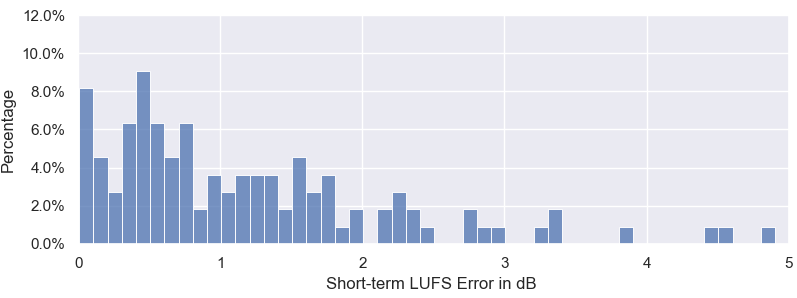
\includegraphics[width=8cm]{File Level Vox.png}
\centering
\caption{Averaged vocal loudness estimation error histogram (file level)}
\end{figure}
\FloatBarrier
Figure 5 shows the distribution of the errors of averaged vocal loudness estimation per file, and the average of all the files is 1.19 dB.

\subsection{Frequency Band Energy Estimation}
\FloatBarrier
\bgroup
\def\arraystretch{1.3}% 
\setlength{\tabcolsep}{3pt}
\begin{table}[h]
\centering
 \caption{Results of the vocal frequency band energy estimation}
 \vspace*{-5mm}
 \begin{center}
\begin{tabular}{l*{13}{c}r}
\hline
\hline
C_f(Hz)$^{\mathrm{*}}$ & 31.5  & 63 & 125  &  250 & 500  & 1K  & 2K & 4K & 8K & 16K \\
\hline
Mean MAE(dB) & 7.96 & \textbf{7.07} &
 \textbf{6.96} & \textbf{6.84} &  \textbf{6.60} &  6.47 & 6.25 & \textbf{5.98} &
 \textbf{5.65} &\textbf{5.49}  \\
 SVR MAE(dB) & \textbf{7.77} & 7.19 &
  7.01 &  7.55  & 6.63  & \textbf{6.38}  & \textbf{6.14} & 6.30 &
  6.20  & 6.23  \\
  \hline
 \multicolumn{4}{l}{$^{\mathrm{*}}$Center frequency.}
\end{tabular}
\egroup
\end{center}
\end{table}
\FloatBarrier

Table II shows the vocal frequency band energy estimation MAEs by the baseline system and the SVR model. The results suggest that the SVR model does not reduce the estimation errors. Because the errors are too large, the frequency band energy estimation is considered invalid for analytical use.
\section{Genre Analysis}

The GTZAN music genre dataset \cite{tzanetakis_essl_cook_2001} is used for vocal loudness analysis. The dataset contains 10 balanced genres, and each genre is represented by 100 mono tracks. Each track is 30 seconds long in 22.05 kHz. Two genres, classical and jazz, are excluded. The averaged relative vocal short-term loudness per track is estimated by the proposed SVR model.

\FloatBarrier
\begin{figure}[h]
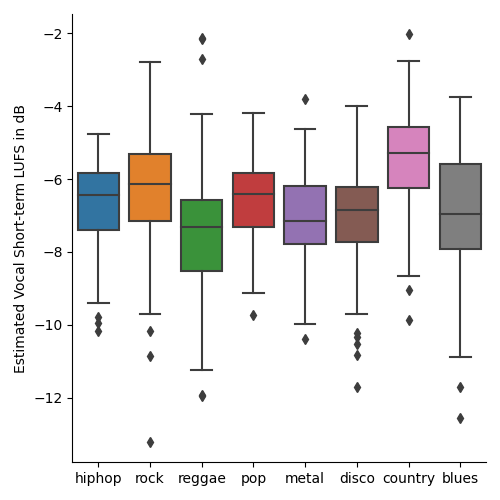
\includegraphics[scale=0.55]{catplot.png}
\centering
\caption{Results of relative vocal loudness analysis by genre}
\end{figure}
\FloatBarrier

\FloatBarrier
\bgrou
\def\arraystretch{1.3}
\setlength{\tabcolsep}{3pt}
%\renewcommand{\setstretch}{0.5}
\begin{table}[h]
\centering
 \caption{Averaged Relative Vocal Loudness by genre}
  \vspace*{-5mm}
 \begin{center}
\begin{tabular}{l*{8}{c}r}
\hline
\hline
Genre & hiphop & rock & reggae  &  pop & metal  & disco  & country & blues  \\
\hline
Loudness(dB) &  -6.69 &  -6.36 &
 -7.58 &-6.52 &  -7.13 &  -7.02 & -5.51 & -6.90  \\

 \hline
\end{tabular}
\egroup
\end{center}
\end{table}
\FloatBarrier

In figure 6, the box plot shows the distribution of the analysis results. Table III shows the average relative vocal loudness against the mixture of each genre. The vocals in country music tend to be louder than in other genres, and reggae music commonly has the vocal track set back more in the mix. 

\section{Conclusion}
This paper proposes the method of using SVR model to estimate the vocal loudness from the mixture signal. This model obtains the MAE of 1.86 dB on vocal loudness estimation. An analysis of vocal loudness by genres using the proposed model shows that the vocal is more present in country music that in other genres.

Future directions of improving the estimation include applying other machine learning models, data augmentation by different mixing ratios, and exploring other audio features. The successful of vocal loudness estimation indicates that the same methodology can be used to estimate the loudness of other music instruments in the mix. As the estimation of vocal frequency band energy shows little success more complex models like DNNs may improve such estimation.





\bibliographystyle{plain}
\bibliography{bibliography.bib}



\end{document}
